%% PNAStmpl.tex
%% Template file to use for PNAS articles prepared in LaTeX
%% Version: Apr 14, 2008


%%%%%%%%%%%%%%%%%%%%%%%%%%%%%%
%% BASIC CLASS FILE
%% PNAStwo for two column articles is called by default.
%% Uncomment PNASone for single column articles. One column class
%% and style files are available upon request from pnas@nas.edu.
%% (uncomment means get rid of the '%' in front of the command)

%\documentclass{pnasone}
\documentclass{pnastwo}

%%%%%%%%%%%%%%%%%%%%%%%%%%%%%%
%% Changing position of text on physical page:
%% Since not all printers position
%% the printed page in the same place on the physical page,
%% you can change the position yourself here, if you need to:

% \advance\voffset -.5in % Minus dimension will raise the printed page on the
                         %  physical page; positive dimension will lower it.

%% You may set the dimension to the size that you need.

%%%%%%%%%%%%%%%%%%%%%%%%%%%%%%
%% OPTIONAL GRAPHICS STYLE FILE

%% Requires graphics style file (graphicx.sty), used for inserting
%% .eps files into LaTeX articles.
%% Note that inclusion of .eps files is for your reference only;
%% when submitting to PNAS please submit figures separately.

%% Type into the square brackets the name of the driver program
%% that you are using. If you don't know, try dvips, which is the
%% most common PC driver, or textures for the Mac. These are the options:

% [dvips], [xdvi], [dvipdf], [dvipdfm], [dvipdfmx], [pdftex], [dvipsone],
% [dviwindo], [emtex], [dviwin], [pctexps], [pctexwin], [pctexhp], [pctex32],
% [truetex], [tcidvi], [vtex], [oztex], [textures], [xetex]

\usepackage{graphicx}
\usepackage[space]{grffile}
\usepackage{latexsym}
\usepackage{textcomp}
\usepackage{longtable}
\usepackage{tabulary}
\usepackage{booktabs,array,multirow}
\usepackage{amsfonts,amsmath,amssymb}
\usepackage{natbib}
\usepackage{url}
\usepackage{hyperref}
\hypersetup{colorlinks=false,pdfborder={0 0 0}}
\usepackage{etoolbox}
\makeatletter
\patchcmd\@combinedblfloats{\box\@outputbox}{\unvbox\@outputbox}{}{%
  \errmessage{\noexpand\@combinedblfloats could not be patched}%
}%
\makeatother
% You can conditionalize code for latexml or normal latex using this.
\newif\iflatexml\latexmlfalse
\providecommand{\tightlist}{\setlength{\itemsep}{0pt}\setlength{\parskip}{0pt}}%

\AtBeginDocument{\DeclareGraphicsExtensions{.pdf,.PDF,.eps,.EPS,.png,.PNG,.tif,.TIF,.jpg,.JPG,.jpeg,.JPEG}}

\usepackage[utf8]{inputenc}
\usepackage[english]{babel}



%%%%%%%%%%%%%%%%%%%%%%%%%%%%%%
%% OPTIONAL POSTSCRIPT FONT FILES

%% PostScript font files: You may need to edit the PNASoneF.sty
%% or PNAStwoF.sty file to make the font names match those on your system.
%% Alternatively, you can leave the font style file commands commented out
%% and typeset your article using the default Computer Modern
%% fonts (recommended). If accepted, your article will be typeset
%% at PNAS using PostScript fonts.


% Choose PNASoneF for one column; PNAStwoF for two column:
%\usepackage{PNASoneF}
%\usepackage{PNAStwoF}

%%%%%%%%%%%%%%%%%%%%%%%%%%%%%%
%% ADDITIONAL OPTIONAL STYLE FILES

%% The AMS math files are commonly used to gain access to useful features
%% like extended math fonts and math commands.

%%%%%%%%%%%%%%%%%%%%%%%%%%%%%%
%% OPTIONAL MACRO FILES
%% Insert self-defined macros here.
%% \newcommand definitions are recommended; \def definitions are supported

%\newcommand{\mfrac}[2]{\frac{\displaystyle #1}{\displaystyle #2}}
%\def\s{\sigma}

%====================================================
% MY PACKAGES
%------------------------
\usepackage{amsmath,amsfonts,amsthm,array,amscd,amssymb,dsfont}
\usepackage{color}
\usepackage{cleveref}%to have automatic 'clever' references that includes the words 'figure', 'equation', etc.
\usepackage{dcolumn} % for stargazer tables from R
%for subfigures with their own captions
\usepackage[font={footnotesize}]{caption}
\usepackage{subcaption}
\usepackage{makecell} %to add additional line breaks inside cell in table
%\renewcommand{\cellalign/theadalign}{tl}
%\renewcommand\theadalign{tl}
%\usepackage{bm}

%====================================================
% MY COMMANDS
%------------------------
\newcommand{\ud}{\mathrm{d}}
\newcommand{\e}{\text{e}}
\newcommand{\mtx}[1]{\mathbf{ #1}}
\newcommand{\tr}[1]{\mathrm{tr\left[\mtx{ #1}\right]}}
\newcommand{\rank}[1]{\mathrm{rank\left[\mtx{ #1}\right]}}
\newcommand{\diag}[1]{\mathrm{diag}\left( #1\right)}
\newcommand{\EE}[1]{\mathrm{E\left[\mtx{ #1}\right]}}
\newcommand{\E}[1]{{\mathrm E}\left[ #1 \right]}
\newcommand{\Var}[1]{\mathrm{Var}\left[ #1 \right]}
\newcommand{\prob}[1]{\mathbb{P}\left [ #1 \right ]}
\newcommand{\probSymbol}{\mathbb{P}}
\newcommand{\indicator}[1]{\mathds{1}_{\{#1\}}}
\renewcommand{\vec}[1]{\mathbf{#1}}
\newcommand{\msun}{\,\mathrm{M}_\odot} 



\newcommand\given[1][]{\:#1\vert\:}
%Which will be manually scalled via, say
%\given[\Big] 


%%%%%%%%%%%%%%%%%%%%%%%%%%%%%%
%% Don't type in anything in the following section:
%%%%%%%%%%%%
%% For PNAS Only:
\contributor{Submitted to Proceedings
of the National Academy of Sciences of the United States of America
\url{www.pnas.org/cgi/doi/10.1073/pnas.0709640104}}
\copyrightyear{2008}
\issuedate{Issue Date}
\volume{Volume}
\issuenumber{Issue Number}
%%%%%%%%%%%%

% Close the \begin{article} auto-opened by Authorea, if the author hasn't done so already
\usepackage{etoolbox}
\newbool{InArticleEnvironment}
\AtBeginEnvironment{article}{\booltrue{InArticleEnvironment}}
\AtEndDocument{\ifbool{InArticleEnvironment}{\end{article}}{}}

\begin{document}

\title{Linking Structure to the Dynamics of Collective Learning}


\author{Andres Gomez-Lievano\affil{1}{Harvard University}, Michele Coscia\affil{2}{Harvard University}, Frank Neffke\affil{3}{Harvard University}, Ricardo Hausmann\affil{4}{Harvard University}}


\contributor{Submitted to Proceedings of the National Academy of Sciences
of the United States of America}

\maketitle

\begin{article}
\selectlanguage{english}
\begin{abstract}
The study of cultural evolution has suggested that culture accumulates
as know-how gets transmitted from group to group, and from generation to
generation. The lack of a firm quantitative formalism that takes into
account the structured process of how this accumulation occurs precludes
the development of a unified view of human development in the past and
in the present. The process of accumulating and coordinating
increasingly complex productive capabilities is still what drives the
economic development of nations, regions and cities, as has been well
documented in many empirical studies. We show here that the Theory of
Economic Complexity presents a basis on which to construct such
formalism. We present a combination of analytical, numerical and
empirical results that illustrate how to characterize the process of
development, providing measurable quantities that can be used to predict
future developments. The emphasis is the quantification of the
collective know-how an economy has accumulated, and what are the
directions in which it is likely to expand. As a case study we consider
data on trade, which provides consistent data on the technological
diversification of 200 countries across more than 50 years. Our results
are relevant for anthropologists, sociologists, and economists
interested in the role of collective know-how as the main determinant of
the success and welfare of a society.%
\end{abstract}%



%\keywords{monolayer | structure | x-ray reflectivity | molecular electronics}

%\abbreviations{SAM, self-assembled monolayer; OTS, octadecyltrichlorosilane}



\section{Introduction}
\label{sec:intro} 
For more than a century the field of anthropology has known that human societies, while highly dynamic, diverse, and idiosyncratic, change diachronically through a series of stages of ``complexification'' \hyperref[csl:1]{(1}; \hyperref[csl:2]{2}; \hyperref[csl:3]{3)}. Recent evidence of across hundreds of societies across thousands of years indeed show support of this \hyperref[csl:4]{(4)}. This particular way of cultural unfolding is the result of two processes: one is the diffusion and transmission of cultural traits across human groups and across generations, while the other is the development (through chance or insight) of more complex traits, which is conditionally enabled by previous developments of less complex traits. Thus, the series of complexification stages of a society is constrained by the current set of cultural traits at their disposal, and by the traits they can acquire from other connected populations. The question of whether modern countries, regions and cities develop through these same processes has not been fully studied and analyzed. Here we develop an analytical framework to analyze such processes, and we present strong evidence that they still stand as the fundamental workings of today's modern societies.

Models of cultural learning must track \emph{how much} societies are learning, but they must track who they learn from; a pupil without a teacher does not learn at all. Hence, one requires a formalism in which we can track both the expansion of collective know-how, and the relative movement of societies regarding what they know.

Models of diffusion of cultural traits have been studied in which $N$ individuals are characterized by $M$ internal traits that can take binary values \hyperref[csl:5]{(5}; \hyperref[csl:6]{6)}. The dynamics in these models are interesting in that individuals acquire traits according to two forces: the tendency to conform and the tendency to keep a consistency between the acquired cultural traits. These dynamical rules have a direct translation to the context of collective learning and economic development. The $M$ cultural traits can be thought of as the different levels of pieces of know-how or productive capabilities a population possesses. There are $N$ different societies, and some dynamical rules that determine how know-how migrates between populations. For example, the tendency to conform would imply that societies tend to acquire the most common capabilities, while the tendency of consistency would imply that societies tend to acquire capabilities most similar to the ones it already has.

Given a set of dynamical rules for how collective know-how evolves in societies, one would like to have a method to quantify \emph{how much} a society knows, and \emph{where} is this collective know-how likely to expand, given how capabilities are likely to accumulate.

The first piece of evidence that the same processes that have shaped cultural evolution for thousands of years are still driving current economic development comes from the nestedness of technological matrices (Fig.~\ref{329606}). Presenting observations and their properties ranked and ordered in such a way to reveal a triangular pattern has been used by many disciplines and for many years. Robert Carneiro imported this analysis to anthropology from psychology more than fifty years ago. It has also been at the center of ecology, and more recently, in the study of the patterns of economic development.\selectlanguage{english}
\begin{figure*}[h]
\begin{center}
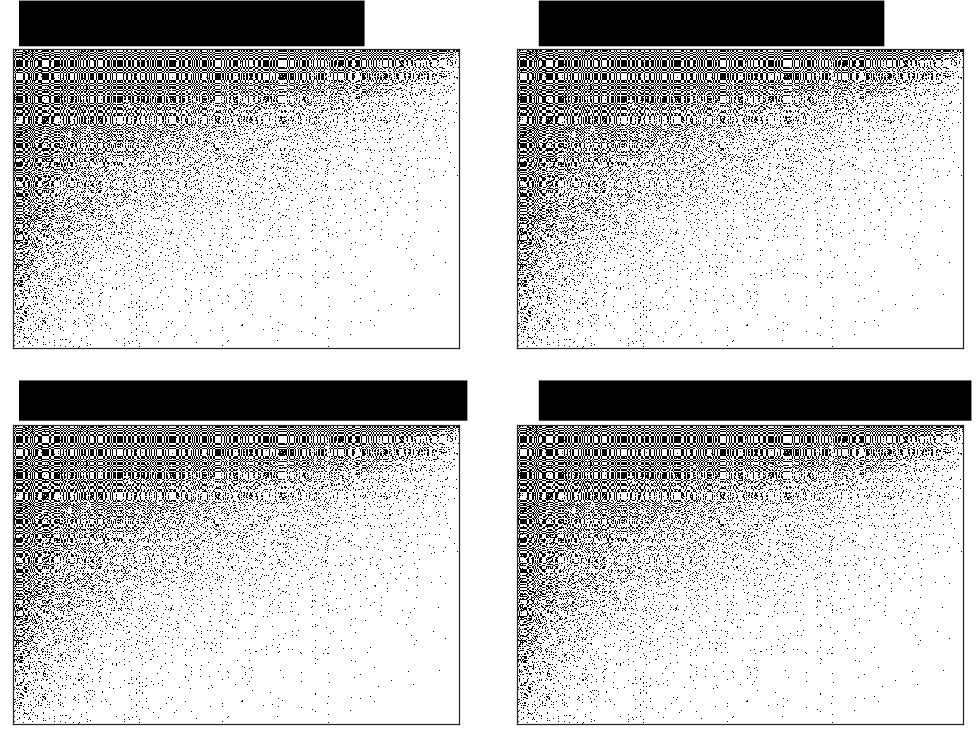
\includegraphics[width=500]{figures/Fig1example/Fig1example}
\caption{{{[}I THINK WE SHOULD START WITH A FIGURE SHOWING THE PATTERN OF
NESTEDNESS (OR LACK THEREOF) IN DIFFERENT TYPES OF ASSOCIATIONS,
DIFFERENT CONTEXTS, DIFFERENT SCALES, AND DIFFERENT TIMES{]}
{\label{329606}}%
}}
\end{center}
\end{figure*}

%One of most important questions in the history of ideas is why are some societies poor and others rich. This is a question for which there is no definite answer yet. 
Among the many theories of socioeconomic evolution, one that has recently gained attention is the Theory of Economic Complexity (TEC) \hyperref[csl:7]{(7}; \hyperref[csl:8]{8}; \hyperref[csl:9]{9}; \hyperref[csl:10]{10}; \hyperref[csl:11]{11}; \hyperref[csl:12]{12}; \hyperref[csl:13]{13)}. TEC emphasizes the flows of tacit know-how as opposed to the flows of ideas, capital or labor. Importantly, TEC emphasizes the combinatorial quality in which qualitatively different pieces of know-how can complement each other, instead of the emphasis traditionally given to knowledge spillovers and the unstructured flows of ideas \hyperref[csl:14]{(14)}. The main take-away from TEC is that societal development is the process of both accumulating, coordinating, and successfully deploying, qualitatively different pieces of productive know-how.


TEC has already proven to be a unifying paradigm. It explains why rich countries are diverse while poor countries are not \hyperref[csl:15]{(15}; \hyperref[csl:16]{16)}, which itself suggests that economic development is process of diversification, not specialization. TEC also suggests an explanation for the phenomenon of urban scaling, whereby larger cities are disproportionately more productive \hyperref[csl:17]{(17}; \hyperref[csl:18]{18)}, and it explains and predicts how do regions (cities, regions or countries) diversify over time \hyperref[csl:19]{(19}; \hyperref[csl:20]{20}; \hyperref[csl:21]{21}; \hyperref[csl:8]{8}; \hyperref[csl:22]{22}; \hyperref[csl:23]{23)}. Central to this paradigm is the question of \emph{how much does a team of individuals know?} In other words, it pushes the research agenda towards the task of quantifying \emph{collective know-how}, and tracking the way it grows, contracts, and is transmitted from society to society and from generation to generation \hyperref[csl:24]{(24}; \hyperref[csl:25]{25)}. 

The notion of collective know-how has to be distinguished from the notion of human capital. Human capital, as it has been used in the literature \hyperref[csl:26]{(26}; \hyperref[csl:27]{27}; \hyperref[csl:28]{28)} is an individual-specific property. In contrast, collective know-how is a group-specific property. Societies may or may not have individuals with high human capital, but still have high collective know-how. That is, a collective of individuals that know is different from a collective that knows. In an extended interpretation, collective know-how can be seen as the body of culture, as is defined in the field of Cultural Evolution \hyperref[csl:29]{(29}; \hyperref[csl:30]{30}; \hyperref[csl:31]{31}; \hyperref[csl:32]{32}; \hyperref[csl:33]{33}; \hyperref[csl:34]{34}; \hyperref[csl:35]{35}; \hyperref[csl:24]{24}; \hyperref[csl:25]{25}; \hyperref[csl:36]{36}; \hyperref[csl:37]{37)}. In this field, the term ``cultural accumulation'' is precisely the process of expanding a society's body of collective know-how. In other words, cultural accumulation is the process of collective learning.

The field of cultural evolution has shown the difficulty of formalizing the notion of collective know-how. Hence, there many ongoing efforts about measuring the collective know-how of groups of individuals \hyperref[csl:38]{(38}; \hyperref[csl:39]{39}; \hyperref[csl:40]{40}; \hyperref[csl:41]{41}; \hyperref[csl:42]{42}; \hyperref[csl:43]{43)}. Conceptually, it is even difficult to define what know-how is. In the literature of cultural evolution, the amount of culture (i.e., the size of a society's collective know-how) is proxied by the number of cultural elements (e.g., the number of technologies and tools in the cultural repertoir). Similarly, one good proxy for the collective know-how of a country is the number of products it exports to the world. Hence, it is reasonable to define know-how as ``the size of all the different things the society knows how to do'', analogously to how we assess students knowledge in standardized tests. However, knowing how to do difficult things counts more than know how to do simple things. Hence, in the reference \hyperref[csl:16]{(16)} an attempt was made to derive a measure of collective know-how, and thus the Economic Complexity Index, or ECI, was born.

In this paper we introduce a new way of understanding how collective know-how expands, is maintained or lost, and we take the opportunity to clarify confusions and controversies surrounding the Economic Complexity Index \hyperref[csl:15]{(15}; \hyperref[csl:16]{16)}, which was expressed mathematically in its current form in the reference \hyperref[csl:44]{(44)}. 




\section{Structure of the argument}
\begin{enumerate}
    \item There are two processes that drive economic diversification:
    \begin{itemize}
        \item ``Learning by resembling''/``Collective imitation'' (migration of know-how and skills)
        \item Innovation (appearance of new skills and new products)
    \end{itemize}
    \item Collective imitation makes the world to have a single community.
    \item Innovation makes the world look nested.
    \item The fact that there is a clear single community suggests that the main mechanism for economic diversification is collective imitation.
    \item In such a world, countries can be clearly laid out in a single dimension that accounts for how embedded in the network they are. That dimension is ECI.
    \item We show, however, that the predictive validity of ECI is not guaranteed if the world has more than one community. Thus ECI is not a universal measure of collective know-how.
    \item We ...
\end{enumerate}

\section{Collective learning by imitation}
\label{sec:learnbyimitation}
Societies evolve in a multidimensional space [Brummitt et al. 2018?]. If each dimension is a capability, a population will change its position in this space as it acquires or loses capabilities. Societies that are complex and developed will occupy many dimensions, while less complex societies will occupy few dimensions. We postulate that the dynamical laws in this space arise from societies trying to copy the most complex societies, and the most complex societies exploring new parts of the technology space by recombinatorial processes.

On one hand, collective imitation we assume occurs by migration of people with specific know-how. The process through which societies resemble each other, and follow one another in this multi-dimensional space, implies that they will start to form a line. In other words, there is a collapse of the dimensionality that societies occupy.

We postulate that a country $c$ compares itself with the rest of countries, and seeks to resemble the richest countries. In other words, we postulate the following state variable that countries try to maximize when looking at a specific country $c'$:
\begin{align}
    U(c, c')=\left(\frac{1}{w_c}\right)S(c, g_{c'})T(g_{c'}),
\label{eq:postulate}
\end{align}
where $g_{c'}$ is the group or community to which country $c'$ belongs, $T(g_{c'})$ is a measure of the \emph{prestige} of the community, and $S(c, g_{c'})$ is a measure of proximity, or similarity, between country $c$ and the community of $c'$. Finally, the term $w_c$ is a measure of wealth, such that if country $c$ is very wealthy, it gets little utility from learning from other countries.

Equation~(\ref{eq:postulate}) posits that country $c$ will try to maximize its resemblance with prestigious (i.e., wealthy) countries. This could be done in many ways, such as adopting the same laws, food, social norms, etc.. However, here we will consider the point of view of production, and more specifically, the ability to be internationally competitive at selling traded goods \hyperref[csl:45]{(45)}. The utility in this case will thus be achieved by copying the products that wealthier countries already are able to export.

In the case of producing goods, we argue that Eq.~(\ref{eq:postulate}) can be re-expressed as
\begin{align}
    U(c, c')=\left(\frac{1}{d_c}\right)\sum_p \frac{M_{c,p}M_{c',p}}{u_p},
\label{eq:diversificationutility}
\end{align}
where $M_{c,p}=1$ is country $c$ exports product $p$, and $u_p$ is the number of countries that export product $p$. Thus, here we are assuming that country $c$ is rewarded by coping from $c'$ rare products.

The maximization of $U(c, c')$ will produce, eventually, a single connected network of countries. However, what do the wealthy countries do? Wealthy countries experiment and tinker with their existing capabilities, and thus build on top of what they already know how to do. This is driven by combinatorial possibilities. And in this way, wealthy countries are exponentially more likely to diversify into products \emph{without} having to copy anybody. However, we do not model this process as a utility maximization, as in Eq.~(\ref{eq:postulate}), because innovation is highly stochastic. Instead, the probability that country $c$ starts to export product $p$ must have two components. First, given by the result of maximizing $U(c, c')$, a country is likely to start to export $p$ if that product is produced by many other countries $c'$. And second, an additional term which has to be an exponential function of the number of capabilities the country has so far accumulated. The movement of poor countries will be mainly driven by the first process of copying, while for wealthy countries the movement will be driven by the second combinatorial process.

These two processes (``imitation of the wealthy'' and ``technological recombination by the wealthy'') we argue will yield as a consequence a nested matrix of countries and products.





\section{Imitation leads to a single community, combinatorics leads to nestedness}
The theoretical hypothesis presented before leads to the prediction that the world should display a nested structure. This structure is captured by the left-eigenvector a matrix which is the projection of the technological matrix, into how much technological overlap there is between societies.

To see this, assume we pause the process of development that we postulated in the last section. And suppose we ask the following question: What are the main two communities of countries, given that they are trying to maximize Eq.~(\ref{eq:diversificationutility})? Given this question, countries get high utilities from belonging to the same communities. Hence, the question of identifying the communities becomes the following mathematical problem:
\begin{align}
    \max \sum_{c,c'} U(c, c') \delta_{g_{c}, g_{c'}}.
\end{align}
That is, we are asking the question of which are the two communities to which countries belong such that at a given instant of time there is high within-community utility. [NOT SURE ALL THIS IS CORRECT/MAKES SENSE/IS THE RIGHT WAY OF PUTTING THIS...].

It turns out, the solution of this maximization problem is to pick a community using the subdominant left-eigenvector of the square matrix whose elements are $[\mtx{C}]_{c,c'}= U(c', c)$. This eigenvector has a specific name in the literature: the Economic Complexity Index. Let us restate this in a different way. The Economic Complexity Index (ECI) that has been used in the literature as a measure of a country's collective know-how is a vectors whose elements quantify the degree to which a country is embedded in one of two communities. Both very positive or very negative values mean nodes highly embedded in their communities. In these terms, previous findings mean that one of the communities tends to grow while the other does not. 

In the next sections we clarify the definitions and properties of the ECI, and we show both numerically and empirically the role of the left-eigenvectors of the matrix $\mtx{C}$ to identify communities, while the right-eigenvectors to quantify the number of capabilities countries have.



\section{Mathematical Definition of ECI and Properties}
\label{sec:ECIdefinition}
The calculation of the ECI starts from the matrix of countries (rows) and the products (columns) they export, $\mtx{M}$. Let this matrix have size $C\times P$. This is a matrix that has been discretized so that $M_{c,p}$ is 1 if the product $p$ is exported in country $c$, and 0 otherwise. From this matrix, one creates two stochastic matrices. First, the right-stochastic (i.e., row-stochastic or row-normalized) transition matrix of ``countries to products'', $$\mtx{R}=\diag{1/\vec{d}}\cdot\mtx{M},$$ and second, the left-stochastic (i.e., column-stochastic or column-normalized) transition matrix of ``products to countries'', $$\mtx{L}=\mtx{M}\cdot\diag{1/\vec{u}},$$ where $\vec{d}=\mtx{M}\cdot\vec{1}$ is the vector that contains the number of products a country exports (i.e., its \emph{diversity}) and where $\vec{u}=\mtx{M}^T\cdot\vec{1}$ is the vector that contains the number of countries from which the product is exported (i.e., its \emph{ubiquity}). We use the notation $\diag{\vec{x}}$ to mean the matrix whose diagonal is the vector $\vec{x}$ and the other values are zero, and $\vec{1}$ to denote a vector of 1's.

Four important characteristics of left-stochastic matrices are worth mentioning, as they will be useful below:\footnote{These properties also hold for right-stochastic matrices, by simply swapping the words ``right'' and ``left''.} 
\begin{enumerate}
    \item A stochastic matrix for discrete markov chain can be represented as a network of nodes connected through directed edges. 
    \item Multiplying on the right of the matrix is the way of \emph{propagating probabilities} through the network of connected nodes. 
    \item Multiplying on the left of the matrix is the way of \emph{averaging some node-specific property} conditioned on standing on each of the nodes and only observing the nodes to which probabilities propagate to.
\end{enumerate}


Let us construct the left-stochastic transition probability matrix of ``countries to countries'' \hyperref[csl:46]{(46)}, $$\mtx{C}=\mtx{L}\cdot\mtx{R}^T.$$ For mathematical convenience, we will assume that the stochastic matrix $\mtx{C}$ is irreducible and aperiodic.\footnote{When $\mtx{C}$ is constructed using real data, it is irreducible since all countries produce at least one product that some other country also produces, and it is aperiodic since, by construction, it has self-loops.} 

Now, let $\vec{l_i}^T$ and $\vec{r_i}$ be the $i$th left-eigenvector and right-eigenvector, respectively, so that the eigenvalues are ordered in decreasing value, $\lambda_1\geq \lambda_2\geq\cdots\geq \lambda_C$. The list of ECIs for countries is defined as the left sub-dominant eigenvector, $\vec{ECI}^T\equiv \vec{l_2}^T$:
\begin{align}
\vec{ECI}^T\cdot \mtx{C}=\lambda_2 \vec{ECI}^T.
\label{eqn:drag}
\end{align}


It is easy to prove that the vector $\vec{d}$ of the diversity of countries is orthogonal to the vector of ECIs, $\vec{ECI}$, once you realize that $\vec{d}$ is actually the dominant right-eigenvector (sometimes referred to as the ``perron'' eigenvector, or just simply, the stationary distribution of the discrete markov chain defined by $\mtx{C}$). Thus, multiplying $\vec{d}$ on the right of $\mtx{C}$, and expanding $\mtx{C}$ into its components,
\begin{align}
    \mtx{C}\cdot\vec{d} &= (\mtx{L}\cdot\mtx{R}^T)\cdot\vec{d}, \nonumber \\
    &= (\mtx{M}\cdot\diag{1/\vec{u}})\cdot(\diag{1/\vec{d}}\cdot\mtx{M})^T\cdot\vec{d}, \nonumber \\
    &= (\mtx{M}\cdot\diag{1/\vec{u}})\cdot(\mtx{M}^T\diag{1/\vec{d}})\cdot\vec{d}, \nonumber \\
    &= (\mtx{M}\cdot\diag{1/\vec{u}})\cdot\mtx{M}^T\cdot\vec{1}, \nonumber \\
    &= (\mtx{M}\cdot\diag{1/\vec{u}})\cdot\vec{u}, \nonumber \\
    &= \mtx{M}\cdot\vec{1}, \nonumber \\
    &= \vec{d}.
\end{align}
Thus, $\vec{d}$ is a right-eigenvector of $\mtx{C}$ associated with the eigenvalue $\lambda_1=1$, which from the Perron-Frobenius theorem one concludes that $\vec{d}$ is the \emph{dominant} right-eigenvector. This means, given classical results from discrete markov chains, that the stationary distribution of the stochastic process defined by $\mtx{C}$ is ${\boldsymbol \pi} = \vec{d}/\sum_c d_c$. Therefore, since left-eigenvectors are orthogonal to right-eigenvectors, $\vec{l_i}^T \cdot \vec{r_j}\propto\delta_{i,j}$, we conclude that $$\vec{ECI}^T\cdot\vec{d}=0,$$ which is a result that had been noted before already in reference \hyperref[csl:47]{(47)}.

All these results apply to the product space matrix as well, $\mtx{P} = \mtx{R}^T\cdot \mtx{L}$. Namely, the sub-dominant left-eigenvector is the list of product complexity indices, PCIs, and the dominant right-eigenvector is proportional to the list of ubiquities.

One of the ways the economic complexity index has been defined is by postulating that products have a complexity, and that the complexity of countries is the average complexity of the products it exports. Conversely, one defines the complexity of the products as the average complexity of the countries where it is exported. It is claimed that this uniquely defines these two vectors. This is true, although any of the left-eigenvectors of the matrices $\mtx{C}$ and $\mtx{P}$ have this precise property. To show it, recall that $\vec{l_i}^T$ and $\vec{r_i}$ are the $i$th left-eigenvector and right-eigenvector of $\mtx{C}$, respectively, and assume denote now $\vec{q_i}^T$ and $\vec{s_i}$ be the $i$th left-eigenvector and right-eigenvector, respectively, of $\mtx{P}$. First, note that
\begin{align}
    \mtx{C}\cdot\mtx{L} &= \left(\mtx{L}\mtx{R}^T\right)\cdot\mtx{L}, \nonumber \\
    &= \mtx{L}\cdot\left(\mtx{R}^T\mtx{L}\right), \nonumber \\
    &= \mtx{L}\cdot \mtx{P}.
\label{eq:CReqRP}
\end{align}
And second, start from the fact that $\lambda_i \vec{l_i}^T = \vec{l_i}^T\cdot \mtx{C}$, and multiply it on the right by the matrix $\mtx{L}$, and then use Eq.~(\ref{eq:CReqRP}):
\begin{align}
    \left(\lambda_i \vec{l_i}^T\right)\cdot\mtx{L}&=\left(\vec{l_i}^T\cdot \mtx{C}\right)\cdot\mtx{L}, \nonumber \\
    \lambda_i \left(\vec{l_i}^T\cdot\mtx{L}\right)&= \vec{l_i}^T\cdot \left(\mtx{C}\cdot\mtx{L}\right), \nonumber \\
    &= \vec{l_i}^T\cdot \left(\mtx{L}\cdot \mtx{P}\right), \nonumber \\
    &= \left(\vec{l_i}^T\cdot \mtx{L}\right)\cdot \mtx{P}, \label{eq:averageonaverage}
\end{align}
which can be re-written as
\begin{align}
    \lambda_i \vec{q_i}^T &= \vec{q_i}^T\cdot \mtx{P}. \label{eq:eigenvecofP}
\end{align}
It is easy to see from Equations~(\ref{eq:averageonaverage}) and (\ref{eq:eigenvecofP}) that if $\vec{l_i}^T$ is a left-eigenvector of $\mtx{C}$, then the vector $\vec{l_i}^T\cdot \mtx{L}$ is the $i$th left-eigenvector of $\mtx{P}$, such that $\vec{q_i}^T = \vec{l_i}^T\cdot \mtx{L}$. Since multiplying on the left of a left-stochastic matrix takes averages, we see that the left-eigenvectors of the product space are the averages of the left-eigenvectors of the country space. In particular, for the complexity indices. Furthermore, we obtain that the eigenvalues of both matrices are the same.\footnote{Since $\mtx{M}$ is typically not square, and there are more products than countries, $P>C$, this results also indicates that the matrix $\mtx{P}$ must have some degenerate eigenvalues, which in turn explains why in the calculation of the PCIs one observes many products with identical values.} This result, obviously, applies to the sub-dominant eigenvectors of both matrices, which are the complexity indices. But the point is that if we use the definition of complexities based on the averages, one has to choose among $\min\{C,P\}$ choices.

Now, the values of ECI have been shown to be positively associated with income levels and income growth of countries \hyperref[csl:16]{(16)}. However, a clear and direct interpretation of the physical meaning of ECI, as the sub-dominant left-eigenvector, and its association with a measure of collective know-how, and its link to economic growth, has been lacking. The reason for this confusion is born out, first, from its flawed interpretation as a linear measure to rank countries, and second, as that interpretation that states that it is that quantity which is the average property of products.

In the next section, we clarify these issues, and we show why it is that ECI is, in fact, a good indicator of the size of the collective know-how of countries. The argument is, however, both obvious and non-trivial. Obvious precisely because of its interpretation as the sub-dominant left-eigenvector, but non-trivial, from the ultimate significance about the emphasis it gives to the underlying process of economic development as a process of collective learning.


\section{ECI as a one-dimensional embedding}
ECI answers the question ``What would be the two main communities of countries?'' given how countries resemble one another in their export baskets. Given the literal interpretation that ECI has received as a physical measure of know-how, and its success predicting economic growth, it would seem hard to demonstrate that ECI has this interpretation. 

Empirically, we can use a trick in order to disentangle the economic aspects of the ECI from its community-related properties. The goal here is to try to use ECI to reveal \emph{geographical communities}, which is accomplished when we add a \emph{geographical dimension} to the matrix $\mtx{M}$: the geographical region of destination where the exporter is exporting a product, i.e, the importer. Hence, we will now have a tensor, $M_{c,i,p}$, where $c$ is the index of the exporter country, $i$ the importer, and $p$ the product traded. 


The following figure (Fig. {\ref{660559}}) shows the
matrix of exporters as rows and importer-product pairs as columns. It
also displays a triangular pattern. To it, we compute the eigenvalues to
have an indication of how many clusters there are. Finally, we plot the
3-dimensional left-eigenspace (top-row of figures in the right 6-panel
plot), and the 3-dimensional right-eigenspace. A clear clustering
pattern emerges, which will become more clear in the numerical exercises
that will follow.\selectlanguage{english}
\begin{figure*}[h]
\begin{center}
\includegraphics[width=500]{figures/Meip-figs/Meip-figs}
\caption{{Real data from the matrix of exporters (rows) vs importer-products
(columns). The density of eigenvalues provides a sense of the number of
communities of exporters by counting the number of large eigenvalues.
The density of the distribution of values of ECI is a further indication
of the number of communities. However, the communities become clear on
the left-eigenspace (each dot is an exporter), which is shown on the
three row-panels. We color the five continents of the exporters,
supporting the idea that exporters belong to the same geographical
communities. The bottom row of 3 panels shows the right-eigenspace,
which we hypothesize provides a measure of the underlying capabilities
of exporters.
{\label{660559}}%
}}
\end{center}
\end{figure*}

\section{Left is for communities, right for capabilities [IS THERE A GAME OF WORDS HERE?]}
\label{sec:communityindex}
The ECI is an index that separates the set of countries in two communities, a core and a periphery. Mathematically, we show that it maximizes a community discovery task. Numerically, we create a synthetic world of several communities, and show that $\vec{ECI}$ is the answer to the question \emph{which of two communities does each country belong to?} Finally, we will show that the role of the ECI becomes evident when we use the flattened export vs. product-importer matrix.

The takeaway from this section is more general, though. We show both left-eigenvectors and right-eigenvectors contain the information about the community structure of the network. However, left-eigenvectors are better about the statistical identification of communities, while the right-eigenvectors are better about measuring capabilities. These two realms are related since the extent to which a country is embedded in a community is itself a measure of the number of capabilities it has. The ultimate reason is Anna Karenina's Principle. Richly diversified countries tend to be all alike, while poorly diversified countries are poorly diversified in their own way.




\subsection{Numerical demonstration}
Recalling that $\mtx{C}$ is a left-stochastic matrix, there are several known results about its spectral properties and their relation to community structure \hyperref[csl:48]{(48}; \hyperref[csl:49]{49)}. 

First, if the nodes of the network are organized in well-defined $k$ clusters, then there are $k-1$ relatively large, nontrivial, eigenvalues, in addition to the dominant eigenvalue with value equal to 1 \hyperref[csl:50]{(50)}. Thus, a heuristic that can be used to infer the number of communities in a network is to count the number of eigenvalues larger than, say, 0.1, in the spectrum of the stochastic matrix. Second, the eigenvectors (both left- and right-eigenvectors) associated with those $k-1$ nontrivial eigenvalues reveal the structure of the clusters. Hence, if the clusters are well-defined, carrying out a $k$-means clustering on the matrix $\mtx{E}_{C\times k-1}$ where the columns are the $k-1$ left-eigenvectors of $\mtx{C}$ would identify the $k$ clusters.

In our case, the left-eigenvectors of $\mtx{C}$ can be used to discover the communities of countries, where the communities are the based on how similar are the export baskets of countries. But as we will show, both left and right-eigenvectors can carry out this function.

As a comparison, we create three $\mtx{M}$ matrices. The first, we created by putting $M_{c,p}=1$ with a probability of 0.6 if $c$ and $p$ belong to the same community, and with probability 0.1 if they belong to different ones. The second way is following \hyperref[csl:51]{(51}; \hyperref[csl:52]{52)}, who hypothesize the interaction between two matrices, $\mtx{{\mathcal C}}$ and $\mtx{{\mathcal P}}$ determines $\mtx{M}$. These underlying matrices are also binary matrices, which can be thought of as the matrix of countries and the capabilities they have on the one hand, and the matrix of products and the capabilities they require to be produced on the other, such that $\mtx{M}=\mtx{{\mathcal C}} \odot \mtx{{\mathcal P}}$, where the operator $\odot$ is a production function operator, which we choose as the Leontief (i.e., a country produces a product if it has all the capabilities required to produce it). Finally, the third way to construct $\mtx{M}$ is from real data. We choose the year 2015, 224 countries and 773 products (SITC4 codes). 




Figure~{\ref{340547}} shows the results from the matrix
filled uniformly, with five communities.
Figure~{\ref{369902}} ~shows the results from the
matrix created based on an underlying structure of capabilities, with
also five communities. Figure~{\ref{583738}} show the
results from real data.

\par\null\selectlanguage{english}
\begin{figure*}[h]
\begin{center}
\includegraphics[width=500]{figures/allfigs-uniform-wide/allfigs-uniform-wide}
\caption{{Example of a matrix connecting countries with products with a uniform
probability. The within-community probability was set at 0.6 and the
between-community probability at 0.1.
{\label{340547}}%
}}
\end{center}
\end{figure*}\selectlanguage{english}
\begin{figure*}[h]
\begin{center}
\includegraphics[width=500]{figures/allfigs-nested-wide/allfigs-nested-wide}
\caption{{Example of a matrix connecting countries with products as it results
from the interaction between the matrix of countries and capabilities,
with the matrix of products and the capabilities required. Within each
community we model a nested pattern in which some countries have many
capabilities and others only a few. We also include the possibility in
which some products can be produced countries regardless of the
community to which they belong.~
{\label{369902}}%
}}
\end{center}
\end{figure*}\selectlanguage{english}
\begin{figure*}[h]
\begin{center}
\includegraphics[width=500]{figures/allfigs-real-wide/allfigs-real-wide}
\caption{{The same exercise as in Figures 1 and 2, but with real data from 2015
using only exporters and their products (see
Fig.~{\ref{660559}} for exporters vs.
importer-products). As can be seen, communities are less clear in this
representation.
{\label{583738}}%
}}
\end{center}
\end{figure*}

As can be seen from Fig. 1 and Fig. 2, the left and right eigenvectors
of the matrix of the country space is helpful in identifying the
communities. The~

\subsection{Mathematical demonstration}
Let us begin by showing that $\vec{ECI}$ is a solution to the following optimization problem:
\begin{align}
    \max \sum_{c'}\frac{1}{d_{c'}}\sum_{c,p} \left(\frac{1_{(c\wedge c'~\text{export}~p)} }{u_p}\right)1_{(c\wedge c'~\text{same community})}
\label{eq:maxproblem}
\end{align}
The free parameters of the maximization are the assignments of countries to one of \emph{two communities}. Let us list the properties of this quantity:
\begin{itemize}
    \item It is higher if countries $c$ and $c'$ export products of low ubiquity (i.e., products that are rare, or difficult to produce).
    \item It is higher if country $c'$ exports few products.
    \item It is higher if countries $c$ and $c'$ export the same products.
    \item It is higher if countries $c$ and $c'$ belong to the same community.
\end{itemize}
Since the only moving part in the quantity is to which of the communities countries belong to, the algorithm will put countries that export the same products together. Furthermore, the algorithm will weigh much more when countries export rare, and presumably difficult to make, products. Finally, each country contributes to the quantity, and since you don't want diverse countries to dominate the sum, you divide by each country's diversity.
[THE ARGUMENT THAT i'D LIKE TO DEVELOP FURTHER IS THAT WHAT THE PREVIOUS PARAGRAPH IS DESCRIBING NOT ONLY THE DEFINITION OF THE ECI; iT IS THE STATE VARIABLE THAT AN ECONOMY IS TRYING TO MAXIMIZE IN THE REAL WORLD. THAT IS, COUNTRIES ARE NOT TRYING TO MAXIMIZE gdp, THEY'RE REALLY (BUT UNCONSCIOUSLY AND IMPLICITLY) TRYING TO MAXIMIZE eci. hENCE, AN ECONOMY IS TRYING TO BELONG TO A COMMUNITY. THIS SHOULD SHELD LIGHT TO DIFFERENT ASPECTS OF THE DIVERSIFICATION PROCESS, AND THUS, IT SHOULD REVEAL THE ``DENSITY REGRESSIONS''.]

Let us define the vector $\vec{s}$, such that $s_c=-1$ if the country $c$ belongs to community 1, and $s_c=1$ if $c$ belongs to community 2. Recalling the definition of the elements $M_{c,p}$ of the matrix $\mtx{M}$, the quantity to maximize in Eq.~(\ref{eq:maxproblem}) can be written as
\begin{align}
    Q&=\sum_{c',c,p} \left(\frac{\mathbb{1}_{(c\wedge c'~\text{export}~p)} }{u_p}\frac{1}{d_{c'}}\right)\mathbb{1}_{(c\wedge c'~\text{same community})}, \nonumber\\
    &=\sum_{c',c,p} \left(\frac{M_{c,p}M_{c',p} }{u_p d_{c'}}\right)\left(\frac{s_{c}s_{c'}+1}{2}\right), \nonumber\\
    &\propto \sum_{c',c,p} s_{c}\left(\frac{M_{c,p}M_{c',p} }{u_p d_{c'}}\right)s_{c'}, \nonumber\\
    &= \vec{s}^T \left(\mtx{M}\cdot\diag{1/\vec{u}})\cdot(\mtx{M}^T\diag{1/\vec{d}}\right) \vec{s}, \nonumber\\
    &=\vec{s}^T \mtx{C} \vec{s}. \label{eq:maxproblemlinalg}
\end{align}
Therefore, the problem is how to choose $\vec{s}$ so as to maximize the expression in Equation~(\ref{eq:maxproblemlinalg}). The strategy for solving this problem is the so-called ``spectral approach'' \hyperref[csl:49]{(49}; \hyperref[csl:53]{53)}, expressing the vector $\vec{s}^T$ as a linear combination of the eigenvectors of $\mtx{C}$. Directly replacing this into Eq.~(\ref{eq:maxproblemlinalg}) will not be useful because the eigenvectors of a non-symmetric matrix are not orthogonal among themselves (only to the other side eigenvectors counterparts). So let us express $\vec{s}$ using both the left and right-eigenvectors, 
\begin{align}
    \vec{s}^T&=\sum_i a_i \vec{l_i}^T, \nonumber\\
    \vec{s}&=\sum_i b_i \vec{r_i}.
\end{align}

%However, since the quantity $Q$ is a scalar, maximizing $\vec{s}^T \mtx{C} \vec{s}$ is equivalent to maximizing $\vec{s}^T \mtx{C}^T \vec{s}$. Using this symmetry, then, we seek to maximize 
Replacing these expressions in Eq.~(\ref{eq:maxproblemlinalg}), we get
\begin{align}
    Q&=\sum_i \lambda_i a_i b_i. 
\end{align}
As has been shown in a number of different instances \hyperref[csl:54]{(54}; \hyperref[csl:55]{55}; \hyperref[csl:53]{53)}, this quantity can be maximized by choosing the $\vec{s}$ to be parallel to eigenvectors with the largest eigenvalues, subject to the constraint that $\vec{s}^T\cdot\vec{s}=C$. In other words, since the maximization problem was originally set as to find the two main communities, one must choose the subdominant eigenvalue, and therefore the corresponding eigenvectors.





\section{Improvements on the Theory of Economic Complexity, and the significance of belonging to a community}
\label{sec:whycommunities}
The Theory of Economic Complexity introduced two main ideas to understand economic development. On the one hand, it proposed that economic development is growth at the extensive margin, or, in less technical terms, economic development is a process of diversification. On the other hand, it introduced the notion that economic development is a historical process structured by technological constraints, in the sense that the extensive margin can be expanded following only a limited number of technological paths and, therefore, its growth depends on previous contingent events that move countries in the right direction. 

These conceptual innovations were accompanied by two analytical tools: the technological space that gives structure to the historical process of development, and the quantification of how much a society knows as a collective through an index of economic complexity. Here we show how our understanding of the physical and mathematical meaning of both innovations allow us to improve both notions. We demonstrate this by showing a superior capacity to predict growth.

\begin{description}
    \item[Hypothesis 1:] After identifying the $k$ communities of countries, the $k$-th dimensional left-eigenspace in which countries can be located (the ECI is one of the dimensions) is useful to predict the \emph{direction} of diversification (i.e., which products will appear next). A better algorithm to calculate the embeddedness of a country in a community may thus predict the appearance of specific products better than before. 
    \item[Hypothesis 2:] After identifying the $k$ communities of countries, the $k$-th dimensional right-eigenspace in which countries can be located (the vector of diversities is one of the dimensions) is a measure of the number of capabilities, and is thus useful to predict levels of wealth. In particular, it is the ``distance to the center of the space'' which is proportional to the number of underlying capabilities of countries. of countries. 
    \item[Hypothesis 3:] Both left- and right-eigenspaces should provide better ways of predicting GDP growth (hence, have a horse race with other alternatives).
\end{description}

The discovery presented in Section~\ref{sec:communityindex} that ECI is a community discovery index is very important piece to understand the process of economic development. In concise terms, it suggests that countries accumulate capabilities by ``looking'' like one another.\selectlanguage{english}
\begin{figure*}[h]
\begin{center}
\includegraphics[width=500]{figures/distance2center/distance2center}
\caption{{The real complexities is the number of capabilities that countries have
in their Cca matrix. The model we have used is Hausmann \& Hidalgo
(2011), but we have included 6 communities. The euclidean distance to
the center of the right-eigenspace is highly correlated with the real
number of capabilities
{\label{657592}}%
}}
\end{center}
\end{figure*}

We test the correlation between the real number of capabilities with
other possible measures, including the original ECI, the Fitness of
Pietronero et al., diversity, among others (see Fig.
{\ref{142689}}).\selectlanguage{english}
\begin{figure*}[h]
\begin{center}
\includegraphics[width=550]{figures/allVSall/allVSall}
\caption{{Correlations scattergrams between pairs of variables that may estimate
the underlying number of capabilities. The best correlation is with~ the
``distance to the center'' of the right-eigenspace (see Fig.
{\ref{657592}}).
{\label{142689}}%
}}
\end{center}
\end{figure*}

\section{Discussion}

{\label{583331}}

The results of this paper can be concisely summarized as follows:
economic development is first and foremost a process of global imitation
with recombinatorial exploration. Imitation gives rise to a single
connected network of countries, and both imitation and recombination
gives rise to the nested structure in which richer countries are more
diverse and build on what less diverse countries know-how to do. The
main significance of this is that humanity as a whole is exploring a
single branch of the technological tree.~

Methodologically, our results imply that identifying the community in
the network to which an economy belongs provides a wealth of information
about the current and future productive capabilities of the economy.

\par\null

\section{Conclusion}

{\label{269251}}

The field of economics has improved of our understanding of markets. In
markets, the two organizing concepts are price and quantity, and the
main organizing mechanism is the equalization of supply and demand. The
Theory of Economic Complexity complements our understanding of economic
systems by emphasizing the role of collective know-how. The
adaptability, welfare, and robustness of an economy all are determined
by the size of the collective know-how of a society. While the
traditional market-centered approach to economics has developed
sophisticated tools to track the flows of value and money, TEC is in the
process of developing better tools and formalisms to track the
expansion, maintenance, and transference, of collective know-how. In
this paper we have build on previous ideas to reinforce the claim that
networks are behind the processes of economic development: networks
highlight collective-level properties like communities. And the main
questions are thus: how do economic communities are formed? Why do nodes
in the same community grow together? Why do we see convergence in income
when nodes belong to the same community (Coscia and
Hausmann!)\hyperref[csl:56]{(56}; \hyperref[csl:57]{57)}?

\selectlanguage{english}
\clearpage
\section*{References}\sloppy
\phantomsection
\label{csl:1}1. Carneiro RL (1970) {A Quantitative Law in Anthropology}. \textit{American Antiquity} 35(04):492–494.

\phantomsection
\label{csl:2}2. Carneiro RL (1962) {Scale Analysis as an Instrument for the Study of Cultural Evolution}. \textit{Southwestern Journal of Anthropology} 18(2):149–169.

\phantomsection
\label{csl:3}3. Chrisomalis S (2006) {Comparing Cultures and Comparing Processes: Diachronic Methods in Cross-Cultural Anthropology}. \textit{Cross-Cultural Research} 40(4):377–404.

\phantomsection
\label{csl:4}4. Turchin P, et al. (2018) {Quantitative historical analysis uncovers a single dimension of complexity that structures global variation in human social organization}. \textit{Proceedings of the National Academy of Sciences} 115(2):E144–E151.

\phantomsection
\label{csl:5}5. Bednar J, Bramson A, Jones-Rooy A, Page S (2010) {Emergent cultural signatures and persistent diversity: A model of conformity and consistency}. \textit{Rationality and Society} 22(4):407–444.

\phantomsection
\label{csl:6}6. Page SE, Sander LM, Schneider-Mizell CM (2007) {Conformity and Dissonance in Generalized Voter Models}. \textit{Journal of Statistical Physics} 128(6):1279–1287.

\phantomsection
\label{csl:7}7. Hausmann R, Klinger B (2006) {Structural Transformation and Patterns of Comparative Advantage in the Product Space}. \textit{{SSRN} Electronic Journal}. doi:10.2139/ssrn.939646.

\phantomsection
\label{csl:8}8. Hidalgo CA, Klinger B, Barabasi A-L, Hausmann R (2007) {The Product Space Conditions the Development of Nations}. \textit{Science} 317(5837):482–487.

\phantomsection
\label{csl:9}9. Arthur WB {Complexity and the Economy}. doi:10.4337/9781781952665.00007.

\phantomsection
\label{csl:10}10. Arthur WB, Polak W (2006) {The evolution of technology within a simple computer model}. \textit{Complexity} 11(5):23–31.

\phantomsection
\label{csl:11}11. Hausmann R, Hidalgo C (2010) {Country Diversification Product Ubiquity, and Economic Divergence}. \textit{{SSRN} Electronic Journal}. doi:10.2139/ssrn.1724722.

\phantomsection
\label{csl:12}12. Bahar D, Hausmann R, Hidalgo C (2012) {International Knowledge Diffusion and the Comparative Advantage of Nations}. \textit{{SSRN} Electronic Journal}. doi:10.2139/ssrn.2087607.

\phantomsection
\label{csl:13}13. Frenken K, Boschma R {Notes on a Complexity Theory of Economic Development}. doi:10.4337/9780857930378.00022.

\phantomsection
\label{csl:14}14. Lucas R (2008) \textit{{Ideas and Growth}} (National Bureau of Economic Research) doi:10.3386/w14133.

\phantomsection
\label{csl:15}15. Hausmann R, Hidalgo CA (2011) {The network structure of economic output}. \textit{Journal of Economic Growth} 16(4):309–342.

\phantomsection
\label{csl:16}16. Hidalgo CA, Hausmann R (2009) {The building blocks of economic complexity}. \textit{Proceedings of the National Academy of Sciences} 106(26):10570–10575.

\phantomsection
\label{csl:17}17. Gomez-Lievano A, Patterson-Lomba O, Hausmann R (2016) {Explaining the prevalence scaling and variance of urban phenomena}. \textit{Nature Human Behaviour} 1(1):0012.

\phantomsection
\label{csl:18}18. Neffke F (2017) {Coworker Complementarity}. \textit{{SSRN} Electronic Journal}. doi:10.2139/ssrn.2929339.

\phantomsection
\label{csl:19}19. Neffke F, Henning M (2012) {Skill relatedness and firm diversification}. \textit{Strategic Management Journal} 34(3):297–316.

\phantomsection
\label{csl:20}20. Neffke FMH, Henning M, Boschma R (2011) {The impact of aging and technological relatedness on agglomeration externalities: a survival analysis}. \textit{Journal of Economic Geography} 12(2):485–517.

\phantomsection
\label{csl:21}21. Neffke F, Henning M, Boschma R (2011) {How Do Regions Diversify over Time? Industry Relatedness and the Development of New Growth Paths in Regions}. \textit{Economic Geography} 87(3):237–265.

\phantomsection
\label{csl:22}22. Cristelli M, Tacchella A, Pietronero L (2015) {The Heterogeneous Dynamics of Economic Complexity}. \textit{{PLOS} {ONE}} 10(2):e0117174.

\phantomsection
\label{csl:23}23. Cristelli M, Tacchella A, Pietronero L (2014) {An Overview of the New Frontiers of Economic Complexity}. \textit{Econophysics of Agent-Based Models} (Springer International Publishing), pp 147–159.

\phantomsection
\label{csl:24}24. Richerson PJ, Boyd R (2004) \textit{{Not By Genes Alone}} (University of Chicago Press) doi:10.7208/chicago/9780226712130.001.0001.

\phantomsection
\label{csl:25}25. Henrich J (2016) \textit{{The Secret of Our Success}} (Princeton University Press) doi:10.1515/9781400873296.

\phantomsection
\label{csl:26}26. Romer P (1989) \textit{{Endogenous Technological Change}} (National Bureau of Economic Research) doi:10.3386/w3210.

\phantomsection
\label{csl:27}27. Romer P (1989) \textit{{Human Capital And Growth: Theory and Evidence}} (National Bureau of Economic Research) doi:10.3386/w3173.

\phantomsection
\label{csl:28}28. Jones C, Romer P (2009) \textit{{The New Kaldor Facts: Ideas Institutions, Population, and Human Capital}} (National Bureau of Economic Research) doi:10.3386/w15094.

\phantomsection
\label{csl:29}29. Feldman MW, Cavalli-Sforza LL (1986) {{TOWARDS} A {THEORY} {FOR} {THE} {EVOLUTION} {OF} {LEARNING}}. \textit{Evolutionary Processes and Theory} (Elsevier), pp 725–741.

\phantomsection
\label{csl:30}30. Cavalli-Sforza L, Feldman M, Chen K, Dornbusch S (1982) {Theory and observation in cultural transmission}. \textit{Science} 218(4567):19–27.

\phantomsection
\label{csl:31}31. Feldman MW, Cavalli-Sforza LL (1984) {Cultural and biological evolutionary processes: gene-culture disequilibrium.}. \textit{Proceedings of the National Academy of Sciences} 81(5):1604–1607.

\phantomsection
\label{csl:32}32. Richerson PJ, Boyd R (2008) {Being human: Migration: An engine for social change}. \textit{Nature} 456(7224):877–877.

\phantomsection
\label{csl:33}33. Badcock C, Boyd R, Richerson PJ (1988) {Culture and the Evolutionary Process.}. \textit{Man} 23(1):204.

\phantomsection
\label{csl:34}34. Boyd R, Richerson PJ, Henrich J (2013) {The Cultural Evolution of Technology}. \textit{Cultural Evolution} (The {MIT} Press), pp 119–142.

\phantomsection
\label{csl:35}35. Griesemer JR, Boyd R, Richerson PJ (1986) {Culture and the Evolutionary Process}. \textit{The Condor} 88(1):123.

\phantomsection
\label{csl:36}36. Muthukrishna M, Henrich J (2016) {Innovation in the collective brain}. \textit{Philosophical Transactions of the Royal Society B: Biological Sciences} 371(1690):20150192.

\phantomsection
\label{csl:37}37. Muthukrishna M, Doebeli M, Chudek M, Henrich J (2017) {The Cultural Brain Hypothesis: How culture drives brain expansion underlies sociality, and alters life history}. doi:10.1101/209007.

\phantomsection
\label{csl:38}38. Mesoudi A (2017) {Pursuing Darwin's curious parallel: Prospects for a science of cultural evolution.}. \textit{Proc Natl Acad Sci U S A}.

\phantomsection
\label{csl:39}39. Kempe M, Lycett SJ, Mesoudi A (2014) {From cultural traditions to cumulative culture: parameterizing the differences between human and nonhuman culture.}. \textit{J Theor Biol} 359:29–36.

\phantomsection
\label{csl:40}40. Legare CH (2017) {Cumulative cultural learning: Development and diversity.}. \textit{Proc Natl Acad Sci U S A}.

\phantomsection
\label{csl:41}41. Kline MA, Boyd R (2010) {Population size predicts technological complexity in Oceania}. \textit{Proceedings of the Royal Society B: Biological Sciences} 277(1693):2559–2564.

\phantomsection
\label{csl:42}42. Vaesen K (2012) {Cumulative Cultural Evolution and Demography}. \textit{{PLoS} {ONE}} 7(7):e40989.

\phantomsection
\label{csl:43}43. Henrich J (2004) {Demography and Cultural Evolution: How Adaptive Cultural Processes Can Produce Maladaptive Losses{\textemdash}The Tasmanian Case}. \textit{American Antiquity} 69(02):197–214.

\phantomsection
\label{csl:44}44. Hausmann R, et al. (2011) \textit{{The atlas of economic complexity: Mapping paths to prosperity}} (Puritan Press).

\phantomsection
\label{csl:45}45. Hausmann R, Hwang J, Rodrik D (2006) {What you export matters}. \textit{Journal of Economic Growth} 12(1):1–25.

\phantomsection
\label{csl:46}46. Yildirim MA, Coscia M (2014) {Using Random Walks to Generate Associations between Objects}. \textit{{PLoS} {ONE}} 9(8):e104813.

\phantomsection
\label{csl:47}47. Kemp-Benedict E (2014) {An interpretation and critique of the Method of Reflections}. \textit{MPRA Paper} 60705.

\phantomsection
\label{csl:48}48. Capocci A, Servedio VDP, Caldarelli G, Colaiori F (2005) {Detecting communities in large networks}. \textit{Physica A: Statistical Mechanics and its Applications} 352(2-4):669–676.

\phantomsection
\label{csl:49}49. Malliaros FD, Vazirgiannis M (2013) {Clustering and community detection in directed networks: A survey}. \textit{Physics Reports} 533(4):95–142.

\phantomsection
\label{csl:50}50. Chauhan S, Girvan M, Ott E (2009) {Spectral properties of networks with community structure}. \textit{Physical Review E} 80(5). doi:10.1103/physreve.80.056114.

\phantomsection
\label{csl:51}51. Hidalgo CA, Hausmann R (2009) {The building blocks of economic complexity}. \textit{Proceedings of the National Academy of Sciences} 106(26):10570–10575.

\phantomsection
\label{csl:52}52. Hausmann R, Hidalgo CA (2011) {The network structure of economic output}. \textit{Journal of Economic Growth} 16(4):309–342.

\phantomsection
\label{csl:53}53. Newman MEJ (2006) {Finding community structure in networks using the eigenvectors of matrices}. \textit{Physical Review E} 74(3). doi:10.1103/physreve.74.036104.

\phantomsection
\label{csl:54}54. Newman MEJ, Girvan M (2004) {Finding and evaluating community structure in networks}. \textit{Physical Review E} 69(2). doi:10.1103/physreve.69.026113.

\phantomsection
\label{csl:55}55. Leicht EA, Newman MEJ (2008) {Community Structure in Directed Networks}. \textit{Physical Review Letters} 100(11). doi:10.1103/physrevlett.100.118703.

\phantomsection
\label{csl:56}56. Coscia M, Cheston T (2017) {Institutions vs. Social Interactions in Driving Economic Convergence:  Evidence from Colombia}. \textit{{SSRN} Electronic Journal}. doi:10.2139/ssrn.2939678.

\phantomsection
\label{csl:57}57. Coscia M, Hausmann R (2015) {Evidence That Calls-Based and Mobility Networks Are Isomorphic}. \textit{{PLOS} {ONE}} 10(12):e0145091.

\end{document}

